\documentclass[a4paper,11pt]{book}
\renewcommand{\familydefault}{\sfdefault}

\usepackage{standalone}
\usepackage[english]{babel}
\usepackage[top=3cm]{geometry}
\usepackage{float}
\usepackage{tabularx}
\usepackage{multirow}
\usepackage{booktabs}
\usepackage{pgfplots}
\usepackage{amsmath}
\usepackage{amssymb}
\usepackage{amsfonts}
\usepackage{siunitx}
\usepackage{tikz}
\usepackage{graphics} % for pdf, bitmapped graphics files
\usepackage{graphicx}
\usepackage{exsheets}
\usepackage{algorithm}
\usepackage{algorithmicx}
\usepackage[noend]{algpseudocode}
\usepackage{hyperref}
\usepackage{enumitem}
\usepackage{filecontents}
\usepackage{multirow}
%\usepackage{showframe}% to show frames
%\ifCLASSOPTIONcompsoc
\usepackage[caption=false, font=normalsize, labelfont=sf, textfont=sf]{subfig}
%\else
%\usepackage[caption=false, font=footnotesize]{subfig}
%\fi    

\usetikzlibrary{patterns,arrows,arrows.meta,calc,intersections,shapes,positioning,decorations.pathreplacing,decorations.markings,decorations.pathmorphing}
\usepackage{multicol}

\sisetup{output-decimal-marker={,},exponent-product=\cdot}

\DeclareSIUnit\atm{atm}
\DeclareSIUnit\dioptre{D}



\def\BState{\State\hskip-\ALG@thistlm}


\definecolor{TitleColor}{rgb}{0.65,0.04,0.07}
\definecolor{NumberColor}{rgb}{0.02,0.04,0.48}

\DeclareInstance{exsheets-heading}{fancy}{default}{
toc-reversed = true ,
indent-first = true ,
vscale = 2 ,
pre-code = \IfInsideQuestionT{\rule{\linewidth}{1pt}} ,
post-code =\IfInsideQuestionT{\rule{\linewidth}{1pt}} ,
subtitle-format = \large\scshape\color{rgb:red,0.65;green,0.04;blue,0.07} ,
number-format = \large\bfseries\color{rgb:red,0.02;green,0.04;blue,0.48} ,
points-format = \itshape ,
join = { number[r,B]title[l,B](.333em,0pt);
title[r,B]subtitle[l,B](1em,0pt)
} ,
attach =
{
main[hc,vc]number[hc,vc](0pt,0pt) ;
main[l,vc]subtitle[hc,vc](\marginparsep,0pt)
}
}



\DeclareInstance{exsheets-heading}{block-subtitle}{default}{
vscale = 2 ,
pre-code = \rule{\linewidth}{1pt} ,
post-code = \rule{\linewidth}{1pt} ,%title-format = \large\scshape\color{TitleColor} ,
number-format = \large\bfseries\color{rgb:red,0.02;green,0.04;blue,0.48} ,
subtitle-format = \large\scshape\color{black} ,
join = {
title[r,B]number[l,B](.333em,0pt) ;
title[r,B]subtitle[l,B](1em,0pt)
} ,
attach = {
main[l,vc]title[l,vc](0pt,0pt) ;
main[r,vc]points[l,vc](\marginparsep,0pt)
},
}

\DeclareQuestionClass{textbook}{textbooks}

\SetupExSheets{
  headings = fancy,
  question/print = true ,
  solution/print = false }
 % counter-format = se.qu ,
%  counter-within = section ,
  %question/pre-hook = \rule{\textwidth}{1pt},


\hypersetup{
	colorlinks = true, 
	breaklinks = true, 
	bookmarks = true,
	bookmarksnumbered = true,
	urlcolor = blue, 
	linkcolor = blue, 
	citecolor=blue,
	linktoc=page, 
	pdftitle={}, 
	pdfauthor={\textcopyright Author}, 
	pdfsubject={}, 
	pdfkeywords={}, 
	pdfcreator={pdfLaTeX}, % PDF Creator
	pdfproducer={IEEE} }





\tikzset{point/.style={circle,fill,black!80,inner sep=0pt,minimum size=#1,opacity=0.9}}
\tikzset{point/.default=3pt}\tikzset{vector/.style={line width=1pt,postaction={decorate,decoration={markings,mark=at position 1 with {\arrow{latex}}}}}}
\tikzset{block/.style={rectangle,fill=black!30,draw,minimum size=#1,opacity=0.9,align=center}}
\tikzset{block/.default=15pt}\tikzset{ball/.style={circle,fill=black!30,draw,minimum size=#1,opacity=0.9}}
\tikzset{ball/.default=5pt}\tikzset{pulley/.style={draw=black,line width=0.2pt,circle,minimum size=#1,inner sep=0pt,fill=black!10}}
\tikzset{pulley/.default=20pt}\tikzset{rod/.style={line width=2pt}}
\tikzset{rope/.style={line width=1pt}}
\tikzset{spring/.style={decorate,decoration={coil,amplitude=5pt,segment length=#1,aspect=0.3}}}
\tikzset{spring/.default=5pt}\tikzset{wall/.style={black!10,pattern=north east lines,opacity=0.3}}
\tikzset{ray/.style={line width=0.8pt,postaction={decorate,decoration={markings,mark=at position 0.5 with {\arrow{>}}}}}}
\tikzset{arrow/.style={-latex}}
\tikzset{object/.style={line width=1pt,orange,-latex}}
\tikzset{image/.style={line width=1pt,blue,-latex}}
\tikzset{doublearrow/.style={<->,>=latex,thick}}
\tikzset{brace/.style={decorate,decoration={brace,amplitude=#1}}}
\tikzset{brace/.default=5pt}




\graphicspath{{images/}} 




\makeatletter
\@addtoreset{question}{section}
\makeatother


\begin{document}
\author{Dr. Muhammed Rushdi \and Asem Alaa}

\title{Measurements and Instrumentation [SBE206A] (Fall 2018)\\ Tutorial 3, 4, \& 5}

\maketitle

\chapter*{Instrument types and performance characteristics (Cont'd)}


\section*{Static characteristics of instruments (Cont'd)}

\begin{itemize}
\item The static characteristics of measuring instruments are concerned only with the steady-state reading that the instrument settles down to, such as accuracy of the reading.
\end{itemize}

\subsection*{Hysteresis}


\begin{figure*}[h!]\label{fig:hysteresis}
\centering
  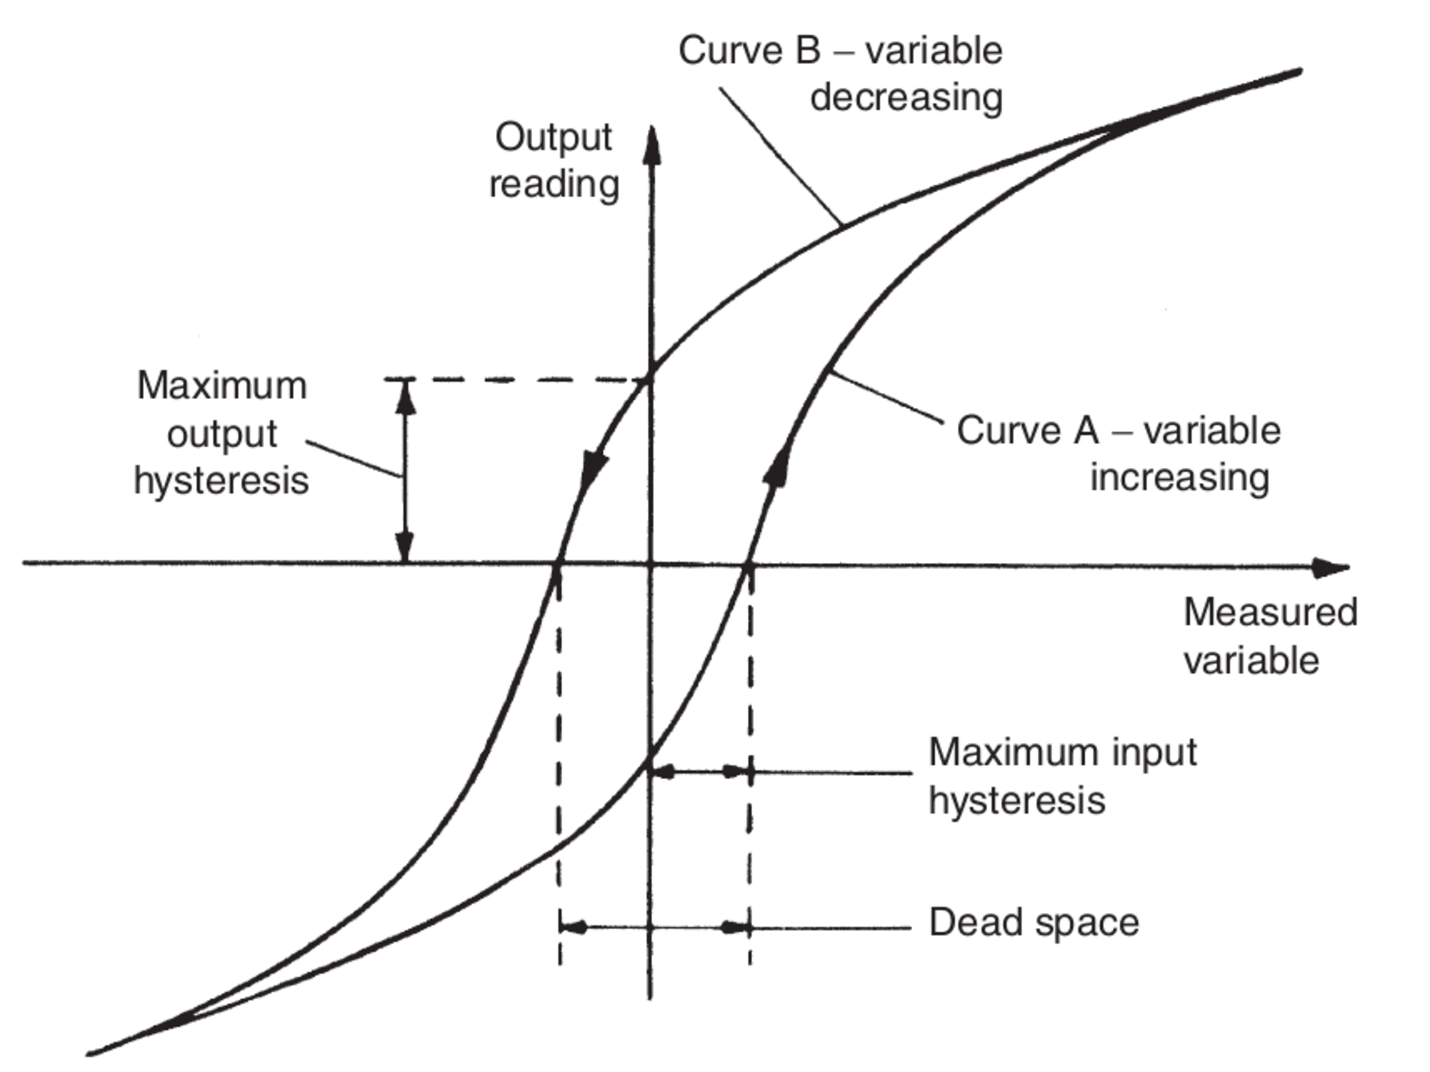
\includegraphics[width=0.7\linewidth]{hysteresis}
  \caption{ Instrument characteristic with hysteresis.} 
\end{figure*}


\subsection*{Dead space}

\begin{figure*}[h!]\label{fig:deadspace}
\centering
  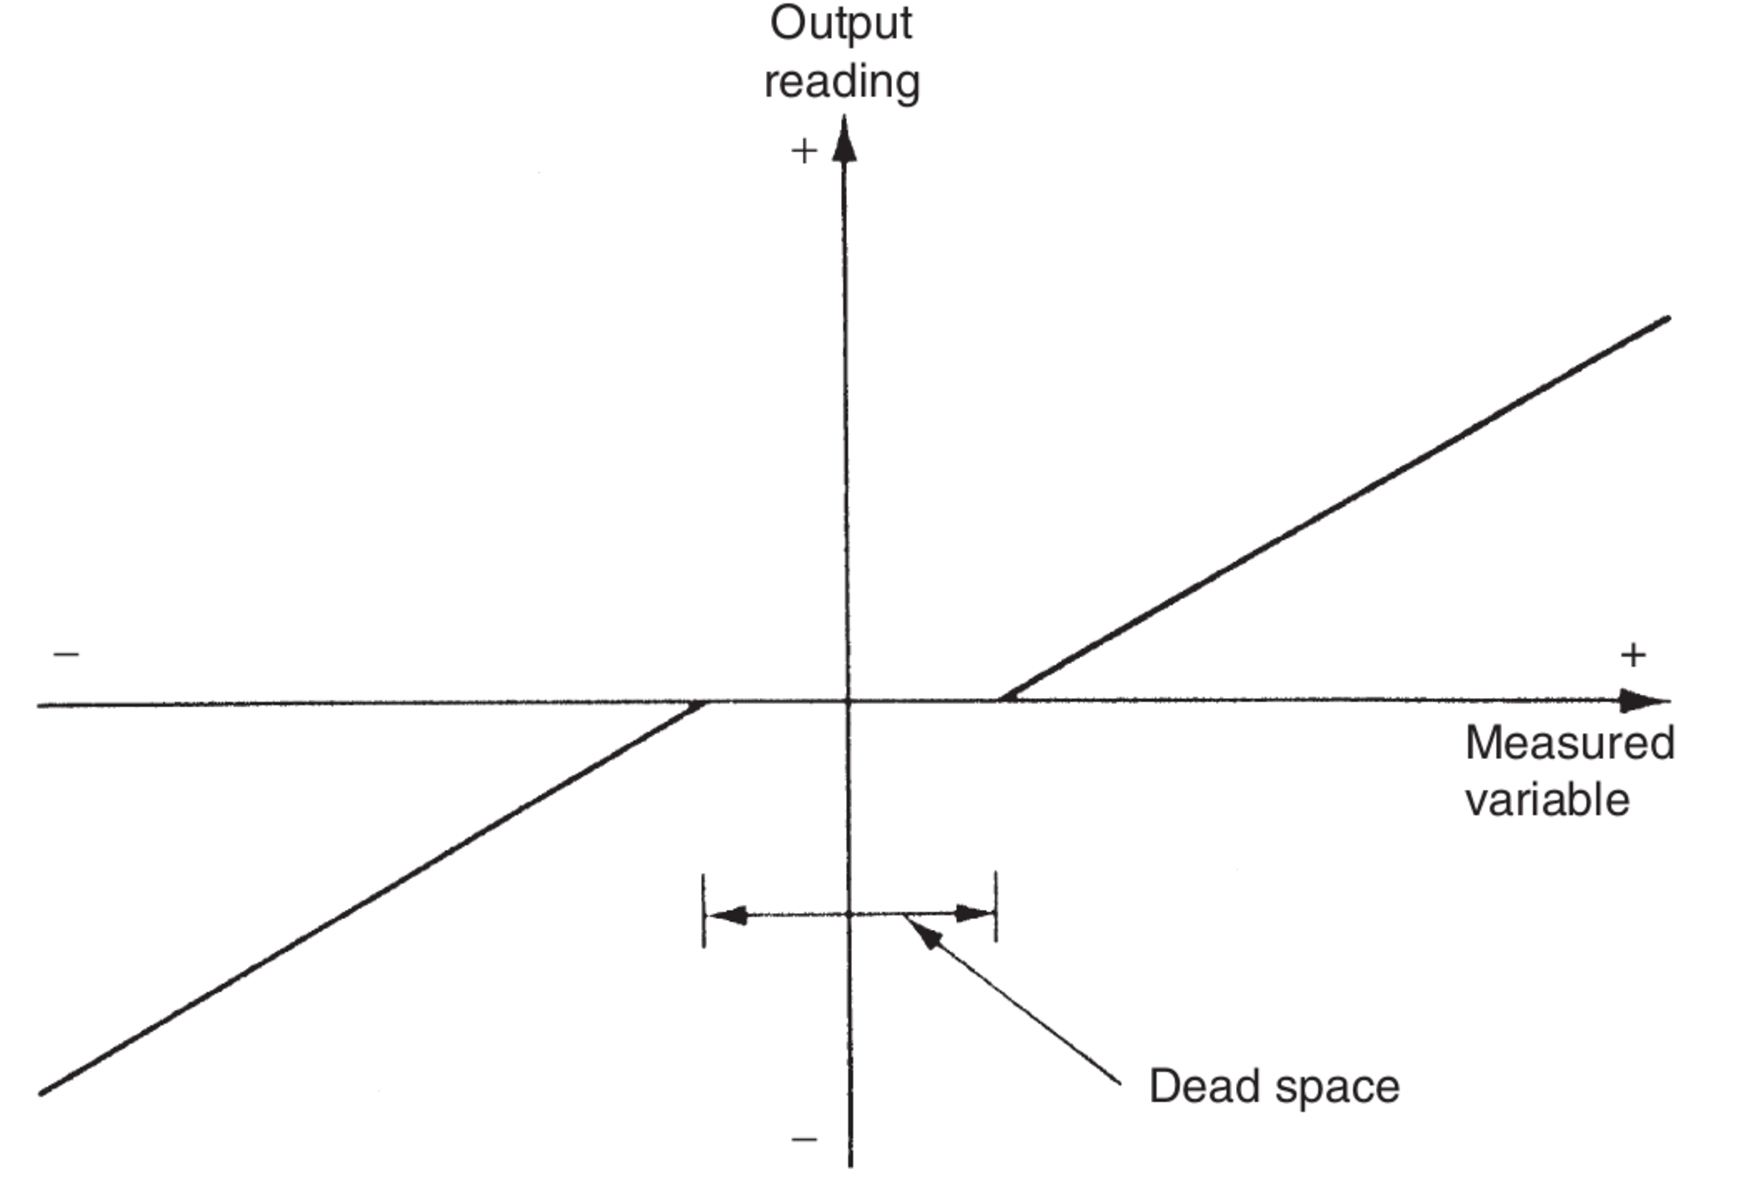
\includegraphics[width=0.7\linewidth]{deadspace}
  \caption{Instrument characteristic with dead space.} 
\end{figure*}

\begin{itemize}
\item Dead space is defined as the range of different input values over which there is no change in
output value.
\item Any instrument that exhibits hysteresis also displays dead space, as marked on Figure \ref{fig:hysteresis}.

\end{itemize}


\section*{Dynamic characteristics of instruments}

\begin{itemize}
\item The dynamic characteristics of a measuring instrument describe its behavior between the time a
measured quantity changes value and the time when the instrument output attains a steady value in
response.
\item In any linear, time-invariant measuring system, the following general relation can be written
between input and output for time $(t)>0$: 
\begin{equation}\label{eqn:dynamic}
a_n \frac{d^{n}q_o}{dt^{n}} + a_{n-1} \frac{d^{n-1}q_o}{dt^{n-1}} + \cdots + a_1 \frac{dq_o}{dt} + a_0 q_o =  b_n \frac{d^{n}q_i}{dt^{n}} + b_{n-1} \frac{d^{n-1}q_i}{dt^{n-1}} + \cdots + b_1 \frac{dq_i}{dt} + b_0 q_i 
\end{equation}
\item If we limit consideration to that of step changes in the measured quantity only, then Equation ~\ref{eqn:dynamic} reduces to:
\begin{equation}\label{eqn:dynamic-reduced}
a_n \frac{d^{n}q_o}{dt^{n}} + a_{n-1} \frac{d^{n-1}q_o}{dt^{n-1}} + \cdots + a_1 \frac{dq_o}{dt} + a_0 q_o =   b_0 q_i 
\end{equation}
\end{itemize}

\subsection*{Zero-order instrument}

If all the coefficients $a_1 \cdots a_n$ other than $a_0$ in Equation \ref{eqn:dynamic-reduced} are assumed zero, then: 

\begin{equation}\label{eqn:zero-order}
a_0 q_o = b_0 q_i ~~\text{or}~~ q_o = b_0 \frac{q_i}{a_0} = K q_i 
\end{equation}

where $K$~ is a constant known as the instrument sensitivity as defined earlier. Figure \ref{fig:zero-order} shows an instrument of zero-order response.

\begin{figure*}[h!]\label{fig:zero-order}
\centering
  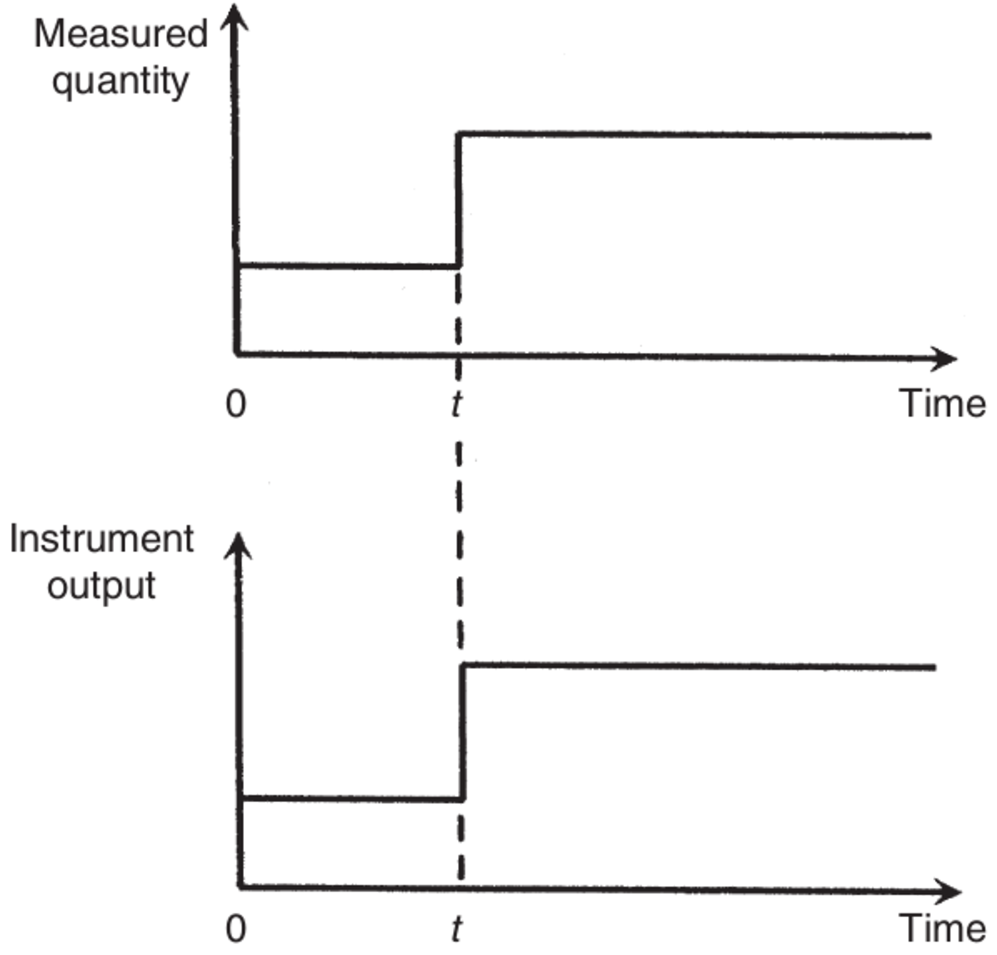
\includegraphics[width=0.7\linewidth]{zero-order}
  \caption{Zero-order instrument characteristic.} 
\end{figure*}


\subsection*{First-order instrument}

If all the coefficients $a_2 \cdots a_n$ except for $a_0$ and $a_1$ in Equation \ref{eqn:dynamic-reduced} are assumed zero, then: 

\begin{equation}\label{eqn:first-order}
a_1 \frac{dq_o}{dt} + a_0 q_o = b_0 q_i  
\end{equation}

Taking the Laplace transform of Equation \ref{eqn:first-order} as a method to solving the differential equation:

\begin{align}
a_1 \left[ s Q_o(s) - q_o(0) \right] + a_0 Q_o(s) &= b_0 Q_i(s) \\ 
( a_1 s + a_0 ) Q_o(s) &= b_0 Q_i(s) + a_1 q_o(0) \\
Q_o(s) &= \frac{ b_0 Q_i(s) + a_1 q_o(0) }{ a_1 s + a_0 } \\
Q_o(s) &= \frac{ K Q_i(s) + \uptau q_o(0) }{ \uptau s + 1} \label{eqn:first-order-laplace}
\end{align}

Where $K = b_0/a_0$ as the static sensitivity and $\uptau = a_1/a_0$ as the time constant of the system.

\begin{figure*}[h!]\label{fig:first-order}
\centering
  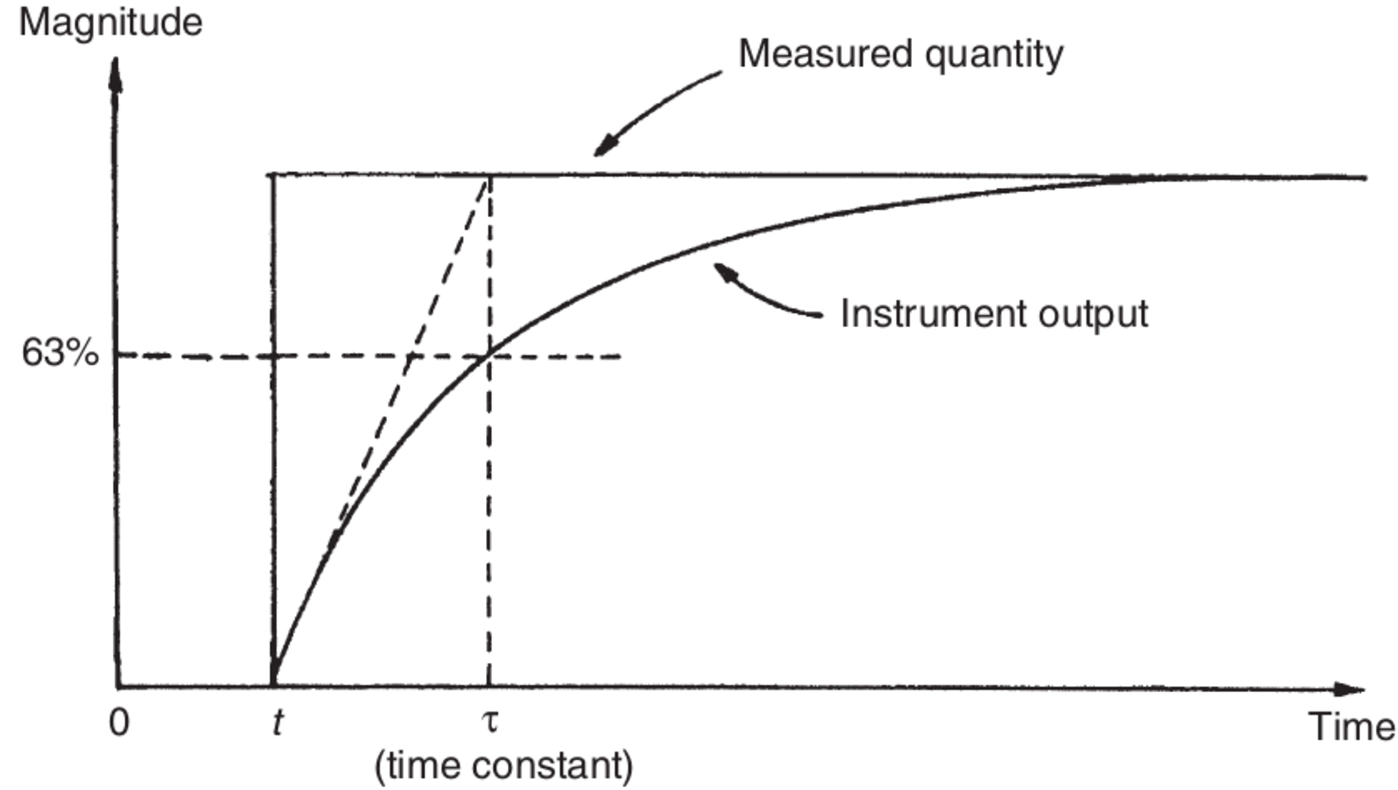
\includegraphics[width=0.7\linewidth]{first-order}
  \caption{First-order instrument characteristic.} 
\end{figure*}

\subsection*{Second-order instrument}

If all the coefficients $a_3 \cdots a_n$ except for $a_0$, $a_1$ and $a_2$ in Equation \ref{eqn:dynamic-reduced} are assumed zero, then: 

\begin{equation}\label{eqn:second-order}
a_2 \frac{d^2q_o}{dt^2} + a_1 \frac{dq_o}{dt} + a_0 q_o = b_0 q_i  
\end{equation}

Taking the Laplace transform of Equation \ref{eqn:second-order} as a method to solving the differential equation:

\begin{equation}
a_2 \left[ s^2 Q_o(s) - s q_o(0) - q_o'(0) \right] + a_1 \left[ sQ_o(s) - q_o(0) \right] + a_0Q_o(s) = b_0 Q_i(s) 
\end{equation}

\begin{align} 
(a_2 s^2 + a_1 s + a_0 ) Q_o(s) &= b_0 Q_i(s) + a_2sq_o(0) + a_2 q_o'(0) + a_1 q_o(0) \\
Q_o(s) &= \frac{ b_0 Q_i(s) + a_2sq_o(0) + a_2 q_o'(0) + a_1 q_o(0) }{ a_2 s^2 + a_1 s + a_0 } \\
Q_o(s) &= \frac{ K \omega_n^2 Q_i(s) + q_o(0)s + q_o'(0) + 2 \eta \omega_n q_o(0) }{ s^2 + 2 \eta \omega_n s + {\omega_n}^2} \label{eqn:second-order-laplace}
\end{align}

Where: \begin{itemize}
\item $K = b_0/a_0$ as the static sensitivity.
\item $\omega_n=\sqrt{\frac{a_0}{a_2}}$ as the undamped natural frequency of the system.
\item $\eta = \frac{a_1 \omega_n}{ 2a_0} = \frac{a_1}{2 \sqrt{a_0a_2}}$ as the \emph{damping ratio} of the system.
\end{itemize} 

\subsection*{Zero initial condition}
To develop intuition about the solution of $q_o(t)$, let's assume that the system is driven by an input of constant quantity (i.e $q_i(t)=const.$ \& $Q_i(s)=\frac{const.}{s}$), and $q_o(t)$ has zero initial value. The system is then described by the following equation:
\begin{equation}\label{eqn:zi-second-order}
Q_o(s) = \frac{ M(s) }{ s(s^2 + 2 \eta \omega_n s + {\omega_n}^2)}
\end{equation}

where $M(s)$ is a polynomial in $s$.

The solution of $q_o(t)$ is subject to computing the roots of the denumerator part $s(s^2 + 2 \eta \omega_n s + {\omega_n}^2)$, where the roots of  $N(s)=(s^2 + 2 \eta \omega_n s + {\omega_n}^2)$ is computed as:
\begin{align}
s_{1,2} &= \frac{-2\eta \omega_n \pm \sqrt{4\eta^2 \omega_n^2 - 4 \omega_n^2}}{2} \\
 &= -\eta \omega_n \pm \omega_n \sqrt{\eta^2 - 1}
\end{align}

which has three cases:
\begin{enumerate}
\item $\eta > 1$: $N(s)$ has real distinct roots, then our system is called highly damped.
\item $\eta = 1$: $N(s)$ has real identical roots, then our system is called critically damped.
\item $\eta < 1$: $N(s)$ has complex roots, then our system is called lightly damped.
\end{enumerate}

\begin{figure*}[h!]\label{fig:second-order}
\centering
  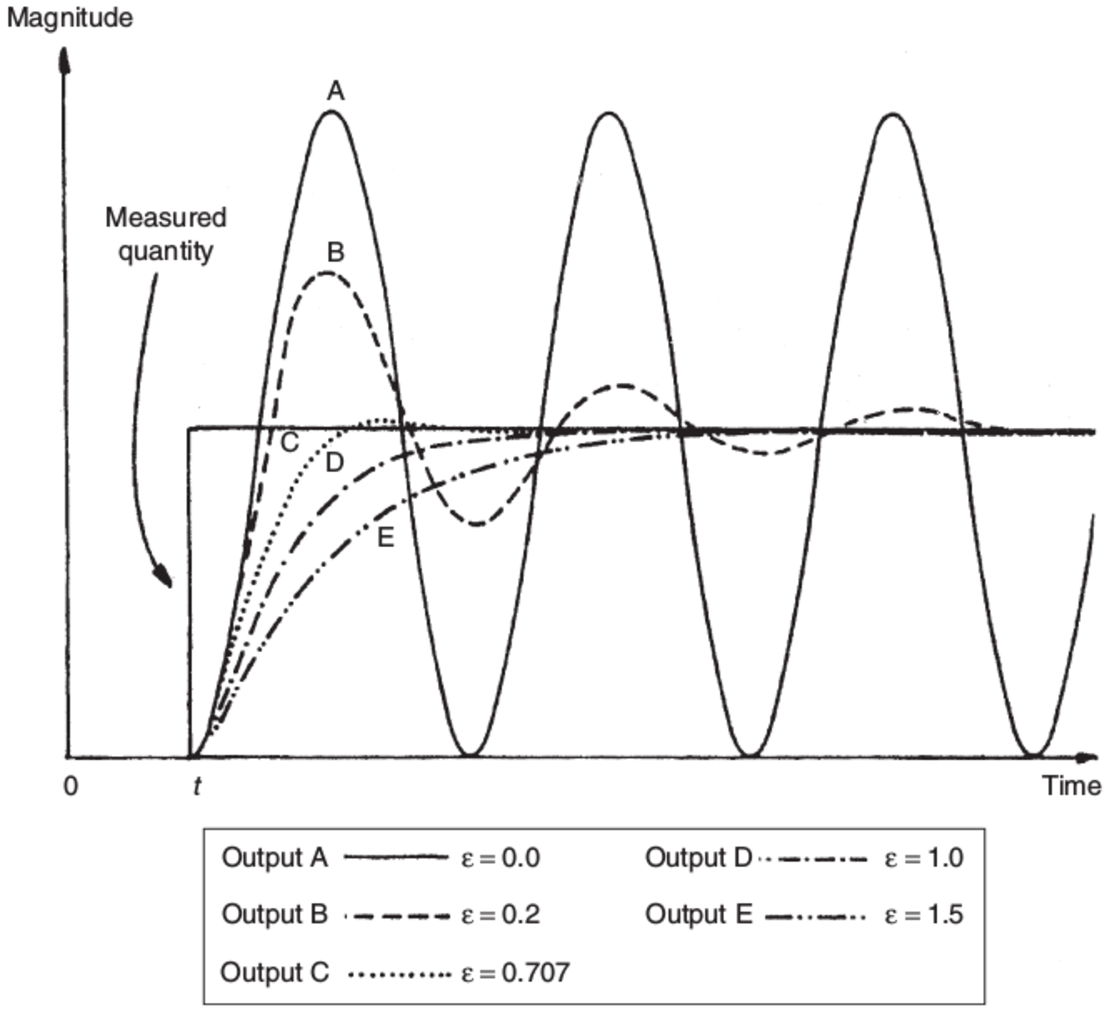
\includegraphics[width=0.7\linewidth]{second-order}
  \caption{Second-order instrument characteristic. } 
\end{figure*}

Figure \ref{fig:second-order} shows a system of second-order reponse with different $\eta$ values.

\subsection*{Case 1: highly damped system ($\eta > 1$)}

The Equation \ref{eqn:zi-second-order} can be factorized as following:
\begin{align*}
Q_o(s)|_{\eta>1} &= \frac{M(s)}{s(s + (\alpha + \beta))(s + (\alpha - \beta)} \\
&= \frac{A}{s} + \frac{B}{s + (\alpha + \beta)} + \frac{C}{s + (\alpha - \beta)}
\end{align*}

where $\beta = \omega_n\sqrt{\eta^2 - 1}$.

and the general solution of $q_o(t)|_{\eta>1}$ becomes:

\begin{equation}
q_o(t)|_{\eta>1} = A + Be^{-(\alpha+\beta)t}+Ce^{-(\alpha-\beta)t}
\end{equation}

\subsection*{Case 2: critically damped system ($\eta = 1$)}

The Equation \ref{eqn:zi-second-order} can be factorized as following:
\begin{align*}
Q_o(s)|_{\eta=1} &= \frac{M(s)}{s(s +\alpha)^2} \\
&= \frac{A}{s} + \frac{B}{s + \alpha} + \frac{C}{(s + \alpha)^2}
\end{align*}


and the general solution of $q_o(t)|_{\eta=1}$ becomes:

\begin{equation}
q_o(t)|_{\eta=1} = A + Be^{-\alpha t}+Cte^{-\alpha t}
\end{equation}

\subsection*{Case 3: lightly damped system ($\eta < 1$)}

The Equation \ref{eqn:zi-second-order} can be expressed as following:
\begin{align*}
Q_o(s)|_{\eta<1} &= \frac{A}{s} + \frac{Bs + C}{s^2 + 2 \eta \omega_n s + {\omega_n}^2} \\
&= \frac{A}{s} + \frac{Bs+C}{(s+\eta \omega_n)^2 + {\omega_n}^2 - \alpha^2} \\
&= \frac{A}{s} + \frac{Bs+C}{(s+\alpha)^2 + \omega_d^2}
\end{align*}

where: 
\begin{itemize}
\item $\alpha=\eta \omega_n$, is called the attenuation coeffiecent.
\item $\omega_d= {\omega_n}^2 - \alpha^2 = \omega_n \sqrt{1-\eta^2}$, is called the damped natural frequency, which is responsible of the oscillation frequency of the system response.
\end{itemize}

and the general solution of $q_o(t)|_{\eta<1}$ becomes:

\begin{equation}
q_o(t)|_{\eta<1} = A + Be^{- \alpha t}\sin(\omega_d t - \phi)
\end{equation}

\section*{Problems}

\begin{question}[subtitle=Example on $1_{\rm st}$-order device]
A balloon is equipped with temperature and altitude measuring instruments and has radio
equipment that can transmit the output readings of these instruments back to ground. The
balloon is initially anchored to the ground with the instrument output readings in steady state.
The altitude-measuring instrument is approximately zero order and the temperature transducer
first order with a time constant of 15 seconds. The temperature on the ground, $T_0$ , is 10 $^{\circ}$C and the temperature $T_x$  at an altitude of x metres is
given by the relation: \\
$T_x = T_0 - 0.01x$

\begin{enumerate}
\item If the balloon is released at time zero, and thereafter rises upwards at a velocity of 5 metres/second, draw a table showing the temperature and altitude measurements reported
at intervals of 10 seconds over the first 50 seconds of travel. Show also in the table the
error in each temperature reading.
\item  What temperature does the balloon report at an altitude of 5000 metres?
\end{enumerate}

\examspace*{10em}

\end{question}
\begin{solution}


\end{solution}

\begin{question}[subtitle=Example on $1_{\rm st}$-order device]
An unmanned submarine is equipped with temperature and depth measuring instruments
and has radio equipment that can transmit the output readings of these instruments back to
the surface. The submarine is initially floating on the surface of the sea with the instrument
output readings in steady state. The depthmeasuring instrument is approximately zero order
and the temperature transducer first order with a time constant of 50 seconds. The water
temperature on the sea surface, $T_0$ , is 20 $^{\circ}$C and the temperature $T_x$ at a depth of x metres is
given by the relation:
$T_x = T_0 - 0.01x$

\begin{enumerate}
\item If the submarine starts diving at time zero, and thereafter goes down at a velocity of 0.5
metres/second, draw a table showing the temperature and depth measurements reported at
intervals of 100 seconds over the first 500 seconds of travel. Show also in the table the error
in each temperature reading.
\item  What temperature does the submarine report at a depth of 1000 metres?
\end{enumerate}

\examspace*{10em}

\end{question}
\begin{solution}


\end{solution}



\begin{question}
Write down the general differential equation describing the dynamic response of a second
order measuring instrument and state the expressions relating the static sensitivity, undamped
natural frequency and damping ratio to the parameters in this differential equation. Sketch
the instrument response for the cases of heavy damping, critical damping and light damping,
and state which of these is the usual target when a second order instrument is being designed.

\examspace*{40em}

\end{question}
\begin{solution}


\end{solution}


\begin{question}[subtitle=Midterm 2014]
The dynamic error in a temperature measurement using a thermometer is 70\% at 3 seconds
after an input step change in temperature. Determine:
\begin{enumerate}
\item the magnitude ratio at 3 seconds,
\item the thermometer’s time constant (in seconds), and
\item the magnitude ratio at 1 second.
\end{enumerate}
\end{question}
\begin{solution}
\end{solution}


\begin{question}[subtitle=Midterm 2017]
A thermocouple is immersed in a liquid to monitor its temperature fluctuations. Assume the thermocouple acts as a first-order system.
\begin{enumerate}
\item In a planned experiment, the thermocouple is to be exposed to a step change in temperature. The
response characteristics of the thermocouple must be such that the thermocouple’s output reaches 95\% of the final temperature within 5 seconds. Assume that the thermocouple’s bead (its sensing element) is spherical with  a density ${\rm \rho = 8000 ~Kg/m^3}$, a specific heat at constant volume ${\rm C_v = 380 ~J/(Kg.K)}$ and a convective heat transfer coefficient $h = 210 ~W/(m^2 K)$. The time constant of the thermocouple is related to those parameters by $\uptau = \frac{\rm \rho d C_v}{6h}$, where $d$ is the diameter of the thermocouple's bead. Determine the \emph{maximum} diameter that the
thermocouple can have and still meet the desired response characteristics.
\item In another experiment on the same thermocouple, the temperature fluctuations (in ${}^\circ C$) vary in time as $T(t) = 50 + 25\cos(4t)$. The output of the thermocouple transducer system $E(t)$ (in mV) is linearly proportional to temperature and has a static sensitivity of $2~ mV/{}^\circ C$. Find the output $E(t)$ (in mV).
\end{enumerate}

\examspace*{30em}

\end{question}
\begin{solution}
\end{solution}


\begin{question}[subtitle=Midterm 2017]
\begin{figure*}[h!]\label{fig:problem1}
\centering
  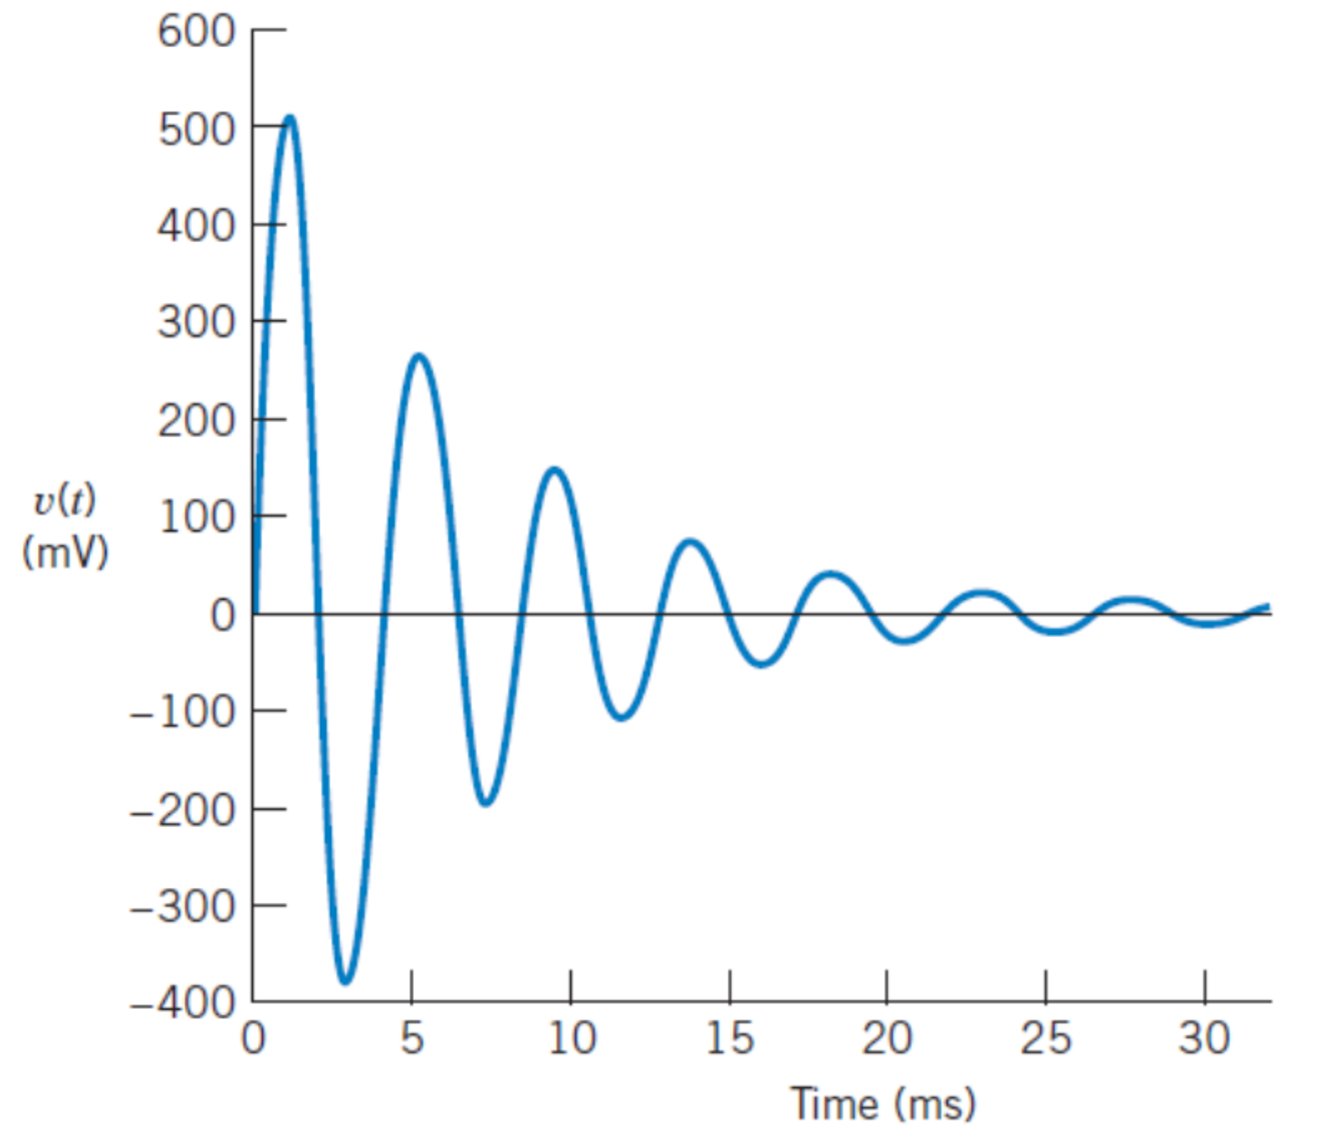
\includegraphics[width=0.7\linewidth]{problem1}
  \caption{Second-order response of the system.} 
\end{figure*}
An instrument is modeled as a parallel RLC circuit whose differential equation is 
\begin{equation*}
\frac{d^2 v(t)}{dt^2} + \frac{1}{RC}\frac{dv(t)}{dt} + \frac{1}{LC}v(t) = 0
\end{equation*}

where $v(t)$ is the capacitor voltage.
The natural response of the instrument is measured
and plotted in the Figure \ref{fig:problem1}. Using this chart, determine:
\begin{enumerate}
\item the damped natural frequency,
\item the damping ratio (using the log-decrement method),
\item the undamped natural frequency,
\item an expression for $v(t)$, and
\item the R, L, and C values.
\end{enumerate}

\examspace*{50em}

\end{question}
\begin{solution}
\end{solution}

\end{document}
